\chapter{Hyperparameter Tuning}
\label{chap:hyperparameter_tuning}
In this chapter, we will incrementally move to an optimized Genetic Algorithm

\section{No Free Lunch Theorem}
No Free Lunch Theorem:
The best hyperparameter settings of a Genetic Algorithm are very problem specific. \cite{kacprzyk_parameter_2007}, \cite{dao_maximising_2016} \todo{More ref}

\section{Start Scenario}

\section{Population}
\label{chap:hyperparameter_tuning:population}
The number of Individuals is of high importance to a genetic algorithm, as has been explained in section \ref{chap:foundation:genetic_algorithm}. Especially considering the limed processing resources available, a suitable population size has to be found. On one hand, a population that is too low might result in less diverse runs of the genetic algorithm, on the other hand, if population is too high, the simulations will become too costly. Considering these points, the first step of the hyper parameter tuning was to find a suitable population size. In the next chapter \ref{chap:hyperparameter_tuning:other_parameter}, we will aim to improve the hyperparamter using a more robust approach.

In order to test for the best population size, the other hyperparameters have to be assumed using an educated guess. While reviewing the literature, trends of general settings for genetic algorithms can be found. However \cite{mills_determining_2015} highlight the inconsistencies between findings, stating to have "uncovered conflicting opinions and evidence regarding key GA control parameters". 

However \cite{grefenstette_optimization_1986} suggests, that "while it is possible to optimize GA control parameters, very good performance can be obtained with a range of GA control parameter settings." 
This is also complimented by findings from \cite{kacprzyk_parameter_2007}: "The key insight from such studies is the robustness of EAs with respect to their parameter settings. Getting “in the ball park” is generally sufficient for good EA performance. Stated another way, the EA parameter “sweet spot” is reasonably large and easy to find [18]. As a consequence most EAs today come with a default set of static parameter values that have been found to be quite robust in practice."

Chosing the right selection method is complicated as well, as discuees by \cite{kacprzyk_parameter_2007}:
"One source of difficulty here is that selection pressure is not as easy to “parameterize” as population size. We have a number of families of selection procedures (e.g, tournament selection, truncation selection, fitness-proportional selection, etc.) to choose from and a considerable body of literature analyzing their differences (see, for example, [19] or [15]), but deciding which family to choose or even which member of a parameterized family is still quite difficult, particularly because of the interacting effects with population size [13]."

Looking at the literature might lead to hyperparameters are used that at least sufficient enough, to get an idea which range for population size is suitable. We will now look at different concrete hyperparameter suggestions from the literature.

\subsection{Suggested hyperparameter from the literature}
\todo{Use best values also from : Using genetic algorithms for automating automated lane-keeping system testing}
\todo{Talk about rules (e.g. 1/n for mut rate...) - look at: Parameter selection in genetic algorithms}
In an often cited thesis by \cite{de_jong_analysis_1975}, the following parameters have been suggested:
GA(50, 0.6, 0.001, 1.0, 7, E) These suggested parameters have been used successfully by various different genetic algorithms \cite{grefenstette_optimization_1986}. 

An extensive study by \cite{mills_determining_2015} which that took over "over 60 numerical optimization problems." into consideration found that "the most effective level settings found for each factor: population size = 200, selection method = SUS, elite selection percentage = 8\%, reboot proportion = 0.4, number of crossover points = 3, mutation rate = adaptive and precision scaling = 1/2 as fine as specified by the user."

\cite{grefenstette_optimization_1986} claim that GA(30, 0.95, 0.01, 1.0, 1, E) and GA(80, 0.45, 0.01, 0.9, 1, P) produced the best results. They also advised against, a mutation rate of over 0.05, suggesting poor performance. Using a low mutation rate is also suggested by \cite{whitley_genetic_1994} and \cite{jinghui_zhong_comparison_2005}. 
On the other hand, \cite{boyabatli_parameter_2004} state, that "Controversial to existing literature on GA, our computational results reveal that in the case of a dominant set of decision variable the crossover operator does not have a significant impact on the performance measures, whereas high mutation rates are more suitable for GA applications."
Other paper also find a relatively high mutation rate useful. \cite{almanee_scenorita_2021} uses genetic algorithms in a similar domain as this thesis. There, a Population of 50, crossover of 0.8 and mut of 0.2 was used. These used params are the same as the default params from deap (pop = 50 CXPB, MUTPB, NGEN = 0.5, 0.2, 4). \todo{cite https://deap.readthedocs.io/en/master/overview.html}

\cite{srinivas_genetic_1994} state, that for a higher population, cross : 0.6, mut: 0.001 and pop: 100 is a good starting point, while a lower population needs higher crossover and mutation rates like this cross: 0.9, mut: 0.01, pop: 30

These next three paper use ANOVA analysis to come a conclusion. \cite{fazal_estimating_2005} recommend:
Migration direction: Forward
Population size: 50 
Fitness scaling function: Rank
Selection function: Tournament
Elite count: 5
Crossover fraction: 0.5
Crossover function: Scattered


\cite{dao_maximising_2016} suggests these values after anova:
Migdirection: forwards
pop size: 200
fitness scaling: rank
selection: roulette
elite count: 1
Crossover prop: 0.7
MutationFunc: Gaussian
Crossover FUnc: two point
hybrid function: none


\cite{assistant_professor_amity_university_jaipur_rajasthan_india_parameter_2019} use these values after anova:
Direction: Forward
Pop: 200 
Fitness Scaling Function: linar Shift
selection: Roulette 
elite count: 10 
Crossover: 0.4 
Mutation: Constraint Dependent 
Crossover function: Heuristi
Hybrid Function: None




\subsection{results}
This now leads to a difficult decision in choosing the right parameters. Based on the extensive research, we will compare population size of 32, 48, 64 and 96. We will compare the different crossover rates: 0.8 and 0.6. For mutation, 0.01 and 0.2 will be discussed. Further we will use tournament selection with 2 and 4.
Each run will be executed 5 times to get rid of randomness and to make the results more robuts. We will run each simulation for 40 Generations.

\begin{figure}[!h]
	\centering
\begin{tabular}{ |l|c||c|c|c|c|  }
	\hline
	\multicolumn{6}{|c|}{Comparison of Population Size - mean(standard deviation)} \\
	\hline
	Settings & Code & 32 & 48 & 64 & 96\\
	\hline
	C: 0.6, M: 0.01, TS: 2   	& A & 3051 (74) & 3016 (85) & 2851(132) & 2871 (57)\\
	C: 0.6, M: 0.01, TS: 4		& B & 3111 (79) & 3021(110) & 3079(103) & 2937(129)\\
	C: 0.6, M: 0.2, TS: 2 		& C & 3062(128) & 3010 (55) & 3002 (76) & 2831(110)\\
	C: 0.6, M: 0.2, TS: 4    	& D & \cellcolor{green}3020 (44) & 2967 (37) & 2891(181) & 2850 (90)\\
	C: 0.8, M: 0.01, TS: 2   	& E & 3063(105) & \cellcolor{green}2892(222) & 2971(108) & 2916(158)\\
	C: 0.8, M: 0.01, TS: 4		& F & 3052(109) & 3049 (96) & 3054 (68) & 2897(117)\\
	C: 0.8, M: 0.2, TS: 2 		& G & 3099(127) & 2940(111) & 2959 (96) & 2869(131)\\
	C: 0.8, M: 0.2, TS: 4    	& H & 3058 (49) & 3005 (84) & \cellcolor{green}2794(173) & \cellcolor{green}2809(105)\\
	\hline
\end{tabular}
\caption{List Settings per Population Size}
\end{figure}


In figure \ref{figure:population:results}, the results per population are plotted. The line is corresponds to the mean, while the bars show the spread (min to max) of all 5 repetitions.
\begin{figure}[H] 
	\label{figure:population:results}
	\includegraphics[width=1\linewidth]{simulations/population/plots/comparison}
	\caption{mean and error bars per population}
\end{figure}


A high spread can be seen when looking at small population sizes. Considering these findings, a population size of 96 was chosen. While such a high value will result in a performance impact, it is important to keep the variation low.


\section{Design of Experiment}
\label{chap:hyperparameter_tuning:other_parameter}

"Design of experiments is also called statistically designed experiments. The purpose of the experiment and data analysis is to find the causeand-effect relationship between the output and experimental factors in a process."\cite{yang_design_2009}

"In a DOE project, each experimental factor will be changed at least once; that is, each factor will have at least two settings."\cite{yang_design_2009}

"If the range of variable is too small, then we may miss lots of useful information. If the range is too large, then the extreme values might give infeasible experimental runs."\cite{yang_design_2009}



"
DOE data analysis can identify significant and insignificant factors by using analysis of variance.
Ranking of relative importance of factor effects and interactions. Analysis of variance (ANOVA) can identify the relative importance of each factor by giving a numerical score.
DOE data analysis can also provide graphical presentations of the mathematical relationship between experimental factors and output, in the form of main-effects charts and interaction charts.
"\cite{yang_design_2009}

In order to tune the hyperparameter of the genetic algorithm, various different strategies can be used. Using automated hyperparamter tuning approaches like "Grid Search", "Bayesian Optimization, "Simmulated Annealing or "Hyperband" might lead to good results with minimal effort (tuning hyperparameter of these search algorithms is still needed), however they require a high number of runs, which is not feasable.\todo{find references} 

Following the conclusion from the previous section \ref{chap:hyperparameter_tuning:population}, a population size of 96 will be used. Executing one run for 30 generations currently takes around 3:50 hours. Although two different workstations were available, the time required to execute the needed number of runs for these automated tests would exceed the available time budged. This is without considering a minimum required number of repetitions to remove randomness in the results.

A different approach called "design of experiment" (DOE), also known as factorial design (\cite{roy_primer_1990}). Each design of experiment has factors, of which each consists of at least two settings, with the actual number of settings being called "levels" (\cite{yang_design_2009}). Design of experiment needs manual expertise to define which factors are possibly of importance and which settings each factor should have, this is a drawback compared to automatic hyperparameter tuning. Afterwards, main effects and interactions can be calculated to find the best settings per factor. Using ANOVA (Analysis of Variance) it is possible to identify the significance of each main effect and interaction. More details on these analysis tools will be provided in section \ref{chap:hyperparameter_tuning:analysis_of_results}.

"Most industrial experiments involve two or more experimental factors. In this case, factorial designs are the most frequently used designs. By a factorial design, we mean that all combinations of factor levels will be tested in the experiment."\cite{yang_design_2009}


In a factorial designs, each possible combination of factor levels needs to be tested. Looking at the proposed factors in table \ref{table:hyperparameter_tuning:settings_to_level}, we would require 1024 runs \todo{generated by minitab (or https://datatab.net/statistics-calculator/design-of-experiments)}.

"Techniques such as fractional (or partial) factorial experiments are used to simplify the experiment. Fractional factorial experiments investigate only a fraction of all possible combinations. This approach saves considerable time and money but requires rigorous mathematical treatment, both in the design of the experiment and in the analysis of the results." \cite{roy_primer_1990} \todo{Is this really the case? What about combinatorial testing? }


\subsection{Taguchi Design}
Various improvements to Design of experiment have been but forward by Dr. Genichi Taguchi, such as reducing the influence of uncontrollable (noise) factors on processes and products and reducing variability. Some of these methods evolve around Signal-to-noise (S/N) analysis and utilizing cost functions to "express predicted improvements from DOE results in terms of expected cost saving" (\cite{roy_primer_1990}). This master thesis will not discuss all of this proposed considerations, for more detail \cite{roy_primer_1990} as well as \cite{yang_design_2009} is highly recommended.

"
There are many similarities between “regular” experimental design and Taguchi’s experimental design. However, in a Taguchi experiment, only the main effects and two-factor interactions are considered. Higher-order interactions are assumed to be nonexistent. In addition, experimenters are asked to identify which interactions might be significant before conducting the experiment, through their knowledge of the subject matter.
"\cite{yang_design_2009}


This masters thesis will mainly utilizes Taguchis orthogonal arrays (OAs), "which represent the smallest fractional factorials and are used for most common experiment designs." (\cite{roy_primer_1990}). This means, that only a fraction of combinations needs to be tested which drastically improves performance. Each row of these matrices contains the factors of one experiment, while the columns correspond the factors \cite{li_taguchi_2021}. 

"Taguchis proposed various different orthogonal arrays which need to be selected based on the individual needs."  \cite{li_taguchi_2021}.

An othogonal array has multiple properties
\todo{Definition orthogonal array}

Using these orthogonal arrays instead of full factorial experiments will lead to needing a much smaller amount of simulation runs (in our case only 16 compared to 1024), while the latter "might not provide appreciably more useful information" \cite{roy_primer_1990}.


"Generally speaking, OA experiments work well when there is minimal interaction among factors; that is, the factor influences on the measured quality objectives are independent of each other and are linear. In other words, when the outcome is directly proportional to the linear combination of individual factor main effects, OA design identifies the optimum condition and estimates performance at this condition accurately. If, however, the factors interact with each other and influence the outcome, there is still a good chance that the optimum condition will be identified accurately, but the estimate of performance at the optimum can be significantly off. The degree of inaccuracy in performance estimates will depend on the degree of complexity of interactions among all the factors."\cite{roy_primer_1990}.

\todo{cons of taguchi arrays: no higher level interactions, Levels are treated as being discrete}

"During many years of applications of factorial design, people have found that higher-order interaction effects (i.e., interaction effects involving three or more factors) are very seldom significant. In most experimental case studies, only some main effects and two-factor interactions are significant."\cite{yang_design_2009}

"In summary, for full factorial experiments, as the number of factors k increases, the number of runs will increase at an exponential rate that leads to extremely lengthy and costly experiments. On the other hand, as k increases, most of data obtained in the full factorial are used to estimate higher-order interactions, which are most likely to be insignificant."\cite{yang_design_2009}

"The values of the factors should be as far away from either side of the current working condition as possible."\cite{roy_primer_1990}.

"After these two steps, the total degrees of freedom of the experimental factors should be determined in the Taguchi experimental design. The degrees of freedom are the relative amount of data needed in order to estimate all the effects to be studied."\cite{yang_design_2009}


Taguchis proposed various different orthogonal arrays which need to be selected based on the individual needs.
When choosing a suitable taguchi ortogonal arrays, we need to take various factors into account, which can make the process tricky. According to \cite{yang_design_2009}, we will have to follow a three step procedure:

\begin{enumerate}
	\item Calculate the total degree of freedom (DOF). 
	\item Following two rules, standard orthogonal array should be selected:
	\begin{enumerate}
		\item Total DOF need to be smaller than the number of runs provided by the orthogonal array.
		\item All required factor level combinations need to be accommodated by the orthogonal array.
	\end{enumerate}
	
	\item Factors have to be assigned using these rules: 
	\begin{enumerate}
		\item In case the factor level does not fit into the orthogonal array, methods such as column merging and dummy level can be used to modify the original array.
		\item Using the linear graph and interaction table, interactions can be defined. 
		\item In case some columns are not assigned, its possible to keep these columns empty.
	\end{enumerate}
\end{enumerate}


For this genetic algorithm, 7 factors (3 Factors of Level 4 and 4 Factors of Level 2) have been selected. Which factors to choose and with which level was done based on experience gained on section \ref{chap:hyperparameter_tuning:population}. In table \ref{table:hyperparameter_tuning:settings_to_level}, every factor with correspondig levels has been listed,

\begin{figure}[H]
	\centering
\begin{tabular}{ |l|c||c|c|c|c|  }
	\hline
	Factors & Code & Level 1 & Level 2 & Level 3 & Level 4\\
	\hline
	CrossoverType 		& A & one point & two point & uniform 0.1 & uniform 0.5\\
	CrossoverProp    	& B & 0.2 & 0.5 & 0.8 & 0.9\\
	MutationProp   		& C & 0.01 & 0.1 & 0.3 & 0.5\\
	ChromosomeType   	& D & Time & Time+NPC & - & -\\
	GeneType			& E & int & dict & - & -\\
	TournamentSize 		& F & 2 & 4 & - & -\\
	IndMutationProp		& G & 0.1 & 0.5 & - & -\\
	\hline
\end{tabular}
\label{table:hyperparameter_tuning:settings_to_level}
\caption{List of Hyperparamters (Factors) matched to a Code and defined settings (Levels)}
\end{figure}


Using this table, we will now find the best standart orthogonal array in section \ref{chap:hyperparameter_tuning:selection_orthogonal_array}. Before doing so, it is important to state, that taguchi allows to test for possible (pre determined) two-level interactions (\cite{yang_design_2009}). Analysing interactions comes at a cost of Degrees of freedom. If we look at the table, an interaction between ChromosomeType and GeneType might be of interest. Using the power of hindsight, we know, that a second two factor interaction is possible within our chosen array, thus we will have a look at the interaction between Tournament Size and IndMutationPropability.


\subsection{Selection of a suitable standart orthogonal array}
\label{chap:hyperparameter_tuning:selection_orthogonal_array}
The total degree of freedom can be quickly calculated using the rules provided by \cite{yang_design_2009}:

\begin{enumerate}
	\item 1 DOF is always used for the overall mean. 
	\item Each factor has a DOF of NumberOfLevels - 1.
	\item Two-factor interactions use this equation to calculate DOF: $(n_{factor1} - 1)(n_{factor2} - 1)$ where $n$ = number of levels.
\end{enumerate}


This leads to the following calculation for the needed 3 Factors of Level 4 and 4 Factors of Level 2 as well as the two interactions between ChromosomeType-GeneType and TournamentSize-IndMutationProp:

\begin{equation} \label{DOF}
	\begin{split}
		DOF & = 1 + 3 * (3 - 1) + 4 * (2 - 1) + 2 * (2 - 1) * (2 - 1) \\
		& = 13
	\end{split}
\end{equation}

A $L_{16}$ array seems suitable to accommodate the required 13 DOF, which can be seen in \ref{table:hyperparameter_tuning:L16_orhtogonal_array}.


\begin{figure}[H]
	\centering
\begin{tabular}{ |c||c|c|c|c|c|c|c|c|c|c|c|c|c|c|c|  }
	\hline
	   & \multicolumn{15}{|c|}{ $L_{16}(2^{15})$ } \\
	NO.& 1 & 2 & 3 & 4 & 5 & 6 & 7 & 8 & 9 & 10& 11& 12& 13& 14&15\\
	\hline
	1  & 1 & 1 & 1 & 1 & 1 & 1 & 1 & 1 & 1 & 1 & 1 & 1 & 1 & 1 & 1\\
	2  & 1 & 1 & 1 & 1 & 1 & 1 & 1 & 2 & 2 & 2 & 2 & 2 & 2 & 2 & 2\\
	3  & 1 & 1 & 1 & 2 & 2 & 2 & 2 & 1 & 1 & 1 & 1 & 2 & 2 & 2 & 2\\
	4  & 1 & 1 & 1 & 2 & 2 & 2 & 2 & 2 & 2 & 2 & 2 & 1 & 1 & 1 & 1\\
	5  & 1 & 2 & 1 & 1 & 1 & 2 & 2 & 1 & 1 & 2 & 2 & 1 & 1 & 2 & 2\\
	6  & 1 & 2 & 2 & 1 & 1 & 2 & 2 & 2 & 2 & 1 & 1 & 2 & 2 & 1 & 1\\
	7  & 1 & 2 & 2 & 2 & 2 & 1 & 1 & 1 & 1 & 2 & 2 & 2 & 2 & 1 & 1\\
	8  & 1 & 2 & 2 & 2 & 2 & 1 & 1 & 2 & 2 & 1 & 1 & 1 & 1 & 2 & 2\\
	9  & 2 & 1 & 2 & 1 & 2 & 1 & 2 & 1 & 2 & 1 & 2 & 1 & 2 & 1 & 2\\
	10 & 2 & 1 & 2 & 1 & 2 & 1 & 2 & 2 & 1 & 2 & 1 & 2 & 1 & 2 & 1\\
	11 & 2 & 1 & 2 & 2 & 1 & 2 & 1 & 1 & 2 & 1 & 2 & 2 & 1 & 2 & 1\\
	12 & 2 & 1 & 2 & 2 & 1 & 2 & 1 & 2 & 1 & 2 & 1 & 1 & 2 & 1 & 2\\
	13 & 2 & 2 & 1 & 1 & 2 & 2 & 1 & 1 & 2 & 2 & 1 & 1 & 2 & 2 & 1\\
	14 & 2 & 2 & 1 & 1 & 2 & 2 & 1 & 2 & 1 & 1 & 2 & 2 & 1 & 1 & 2\\
	15 & 2 & 2 & 1 & 2 & 1 & 1 & 2 & 1 & 2 & 2 & 1 & 2 & 1 & 1 & 2\\
	16 & 2 & 2 & 1 & 2 & 1 & 1 & 2 & 2 & 1 & 1 & 2 & 1 & 2 & 2 & 1\\
	\hline
\end{tabular}
\label{table:hyperparameter_tuning:L16_orhtogonal_array}
\caption{ $L_{16}(2^{15})$ Taguchi ortohogonal array taken from \cite{roy_primer_1990}}
\end{figure}


This graph now needs to be fitted to the needed factors. 4 Level Factors need more space which will be generated using column merging, while interactions need to be assigned as well.
For this, either an interaction table or linear graphs of this $L_{16}$ array can be used (\cite{roy_primer_1990}, \cite{nazandanacioglu_taguchi_2005}). 
The linear graph approach is straight forward and will be selected. While there are multiple linear graphs for $L_{16}$ array, the following graph has the best fit for the requirements from table \ref{table:hyperparameter_tuning:settings_to_level}. If no graph with the perfect fit is found, theses graphs can be modified as well, as described by \cite{nazandanacioglu_taguchi_2005}


"In each of Taguchi’s orthogonal arrays, there are one or more accompanying linear graphs. A linear graph is used to illustrate the interaction relationships in the orthogonal array."\cite{yang_design_2009}

\begin{figure}[H]
	\centering
\begin{tikzpicture}
	% Define 1 2 3
	\node (Node2) at (0,0) {2};
	\node (Middle12) at (0,1) {};
	\node (Eclipse12) at (-0.8,0) {};
	\node (Node1) at (0,2) {1};
	
	\draw (Node2) -- node[midway, right] {3} (Node1);
	
	
	% Define 4 8 12
	\node (Node8) at (2,0) {8};
	\node (Middle84) at (2,1) {};
	\node (Eclipse84) at (1.2,0) {};
	\node (Node4) at (2,2) {4};
	
	\draw (Node8) -- node[midway, right] {12} (Node4);
	
	% Define 5 15 10
	\node (Node10) at (4,0) {10};
	\node (Middle105) at (4,1) {};
	\node (Eclipse105) at (3.2,0) {};
	\node (Node5) at (4,2) {5};
	
	\draw (Node10) -- node[midway, right] {15} (Node5);
	
	% Define 7 9 14
	\node (Node9) at (6,0) {9};
	\node (Node7) at (6,2) {7};
	
	\draw (Node9) -- node[midway, right] {14} (Node7);
	
	
	% Define 6 11 13
	\node (Node11) at (8,0) {11};
	\node (Node6) at (8,2) {6};
	
	\draw (Node11) -- node[midway, right] {13} (Node6);
\end{tikzpicture}
\caption{ Linear Graph of $L_{16}(2^{15})$ taken from \cite{yang_design_2009}}
\end{figure}


In a taguchi linear graph, the nodes as well as the ?Lines? both represent collumns in the orthogonal array. An interaction between to columns that are represented as nodes "comes out to" to the connecting line column \cite{taguchi_taguchis_2005}. This is usefull for both analyzing interactions between columns as well as combining (mergin) interacting columns in case a higher factor is needed.

\paragraph{Column Merging}
A, B and C are both 4 level factors. The currently selected orthogonal only fits 2 level factors. Using column merging, it is possible to extend columns to fit into the given requirements.

"A four-level column is easily prepared from three two-level columns that are part of an interacting group of columns."\cite{roy_primer_1990}

"Steps 1. From the linear graph for L8, select a set of three interacting columns (Figure 5-9). Example: columns 1, 2, and 3. 2. Select any two columns. Suppose 1 and 2 are selected. 3. Combine the two columns row by row, by following the rules of Table 5-19, to get a combined column such as shown in Table 5-17. Replace the original columns 1, 2, and 3 by the new column that has just been prepared."\cite{roy_primer_1990}

"The first three columns of an L8 can be combined to produce a four-level column following the procedure previously described. Step 1. Start with an original L8 and select a set of three interacting columns, say 1, 2, and 3. Step 2. Ignore column 3 (Table 5-21). Step 3. Combine column 1 and 2 into a new column. Follow the procedure as shown by Tables 5-22 and 5-23. Step 4. Assign the four-level factor to this new column and the others to the remaining original two-level columns, as shown in Tables 5-24 and 5-25."\cite{roy_primer_1990}


"The column merging method merges several low-level columns into a high-level column."\cite{yang_design_2009}


\begin{figure}[H]
	\centering
	\begin{tabular}{ |ccccccc|  }
		\hline
		\multicolumn{3}{|c}{ OLD COLUMN } & & & & NEW COLUMN \\
		\hline
		& 1 & 1 & & -> & & 1\\
		& 1 & 2 & & -> & & 2\\
		& 2 & 1 & & -> & & 3\\
		& 2 & 2 & & -> & & 4\\
		\hline
	\end{tabular}
	\caption{Rules taken from \cite{roy_primer_1990}}
	\label{table:hyperparameter_tuning:merging_rules}
\end{figure}

\paragraph{Assigning Interactions}
An interaction between DE is might be possible. As we still have some unused space in the graph, we will also look at the interaction of FG. \todo{Go over notes from paper and explain this}


\begin{figure}[H]
	\centering
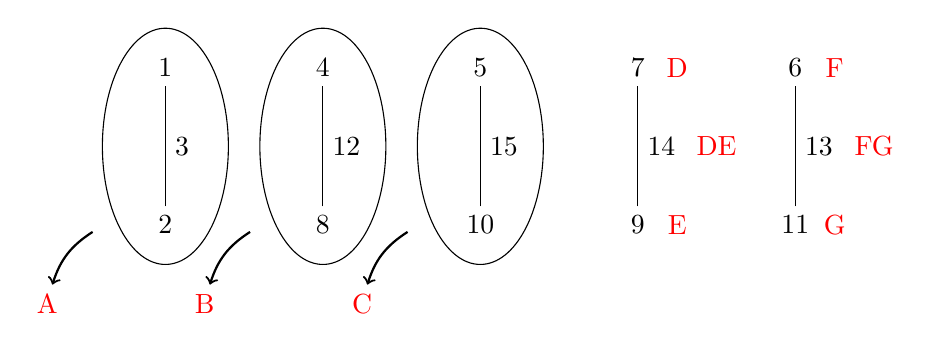
\begin{tikzpicture}
	% Define 1 2 3
	\node (Node2) at (0,0) {2};
	\node (Middle12) at (0,1) {};
	\node (Eclipse12) at (-0.8,0) {};
	\node (Node1) at (0,2) {1};
	\node[red] (A) at (-1.5, -1) {A};

	\draw (Node2) -- node[midway, right] {3} (Node1);
	\draw (Middle12) ellipse (0.8cm and 1.5cm);
	\draw[->, thick] (Eclipse12) to[bend right=20] (A);
	
	
	% Define 4 8 12
	\node (Node8) at (2,0) {8};
	\node (Middle84) at (2,1) {};
	\node (Eclipse84) at (1.2,0) {};
	\node (Node4) at (2,2) {4};
	\node[red] (B) at (0.5, -1) {B};
	
	\draw (Node8) -- node[midway, right] {12} (Node4);
	\draw (Middle84) ellipse (0.8cm and 1.5cm);
	\draw[->, thick] (Eclipse84) to[bend right=20] (B);
	
	% Define 5 15 10
	\node (Node10) at (4,0) {10};
	\node (Middle105) at (4,1) {};
	\node (Eclipse105) at (3.2,0) {};
	\node (Node5) at (4,2) {5};
	\node[red] (C) at (2.5, -1) {C};
	
	\draw (Node10) -- node[midway, right] {15} (Node5);
	\draw (Middle105) ellipse (0.8cm and 1.5cm);
	\draw[->, thick] (Eclipse105) to[bend right=20] (C);
	
	% Define 7 9 14
	\node (Node9) at (6,0) {9};
	\node (Node7) at (6,2) {7};
	\node[red] (E) at (6.5,0) {E};
	\node[red] (D) at (6.5,2) {D};
	\node[red] (DE) at (7,1) {DE};
	
	\draw (Node9) -- node[midway, right] {14} (Node7);
	
	
	% Define 6 11 13
	\node (Node11) at (8,0) {11};
	\node (Node6) at (8,2) {6};
	\node[red] (G) at (8.5,0) {G};
	\node[red] (F) at (8.5,2) {F};
	\node[red] (FG) at (9,1) {FG};
	
	\draw (Node11) -- node[midway, right] {13} (Node6);
\end{tikzpicture}
\caption{Modified Linear Graph to fit our needs}
\end{figure}


Combining columns 1 2 3 to A, 4 8 12 to B and 5 10 15 to C using rules defined by table \ref{table:hyperparameter_tuning:merging_rules} is done in \ref{table:hyperparameter_tuning:merging_columns}.

\begin{figure}[H]
	\centering
	\begin{tabular}{ |c||cccc|cccc|cccc|  }
		\hline
		NO.& 1 & 2 & & \sout{3} & 4 & 8 & &  \sout{12} & 5 & 10 & &  \sout{15}\\
		\hline
		1  & \multicolumn{4}{c}{\sout{1 1} > 1 } & \multicolumn{4}{|c|}{\sout{1 1} > 1 } & \multicolumn{4}{c|}{\sout{1 1} > 1 }\\
		2  & \multicolumn{4}{c}{\sout{1 1} > 1 } & \multicolumn{4}{|c|}{\sout{1 2} > 2 } & \multicolumn{4}{c|}{\sout{1 2} > 2 }\\
		3  & \multicolumn{4}{c}{\sout{1 1} > 1 } & \multicolumn{4}{|c|}{\sout{2 1} > 3 } & \multicolumn{4}{c|}{\sout{2 1} > 3 }\\
		4  & \multicolumn{4}{c}{\sout{1 1} > 1 } & \multicolumn{4}{|c|}{\sout{2 2} > 4 } & \multicolumn{4}{c|}{\sout{2 2} > 4 }\\
		5  & \multicolumn{4}{c}{\sout{1 2} > 2 } & \multicolumn{4}{|c|}{\sout{1 1} > 1 } & \multicolumn{4}{c|}{\sout{1 2} > 2 }\\
		6  & \multicolumn{4}{c}{\sout{1 2} > 2 } & \multicolumn{4}{|c|}{\sout{1 2} > 2 } & \multicolumn{4}{c|}{\sout{1 1} > 1 }\\
		7  & \multicolumn{4}{c}{\sout{1 2} > 2 } & \multicolumn{4}{|c|}{\sout{2 1} > 3 } & \multicolumn{4}{c|}{\sout{2 2} > 4 }\\
		8  & \multicolumn{4}{c}{\sout{1 2} > 2 } & \multicolumn{4}{|c|}{\sout{2 2} > 4 } & \multicolumn{4}{c|}{\sout{2 1} > 3 }\\
		9  & \multicolumn{4}{c}{\sout{2 1} > 3 } & \multicolumn{4}{|c|}{\sout{1 1} > 1 } & \multicolumn{4}{c|}{\sout{2 1} > 3 }\\
		10 & \multicolumn{4}{c}{\sout{2 1} > 3 } & \multicolumn{4}{|c|}{\sout{1 2} > 2 } & \multicolumn{4}{c|}{\sout{2 2} > 4 }\\
		11 & \multicolumn{4}{c}{\sout{2 1} > 3 } & \multicolumn{4}{|c|}{\sout{2 1} > 3 } & \multicolumn{4}{c|}{\sout{1 1} > 1 }\\
		12 & \multicolumn{4}{c}{\sout{2 2} > 3 } & \multicolumn{4}{|c|}{\sout{2 2} > 4 } & \multicolumn{4}{c|}{\sout{1 2} > 2 }\\
		13 & \multicolumn{4}{c}{\sout{2 2} > 4 } & \multicolumn{4}{|c|}{\sout{1 1} > 1 } & \multicolumn{4}{c|}{\sout{2 2} > 4 }\\
		14 & \multicolumn{4}{c}{\sout{2 2} > 4 } & \multicolumn{4}{|c|}{\sout{1 2} > 2 } & \multicolumn{4}{c|}{\sout{2 1} > 3 }\\
		15 & \multicolumn{4}{c}{\sout{2 2} > 4 } & \multicolumn{4}{|c|}{\sout{2 1} > 3 } & \multicolumn{4}{c|}{\sout{1 2} > 2 }\\
		16 & \multicolumn{4}{c}{\sout{2 2} > 4 } & \multicolumn{4}{|c|}{\sout{2 2} > 4 } & \multicolumn{4}{c|}{\sout{1 1} > 1 }\\
		\hline
	\end{tabular}
	\caption{Building 4 Level columns from 2 Level columns}
	\label{table:hyperparameter_tuning:merging_columns}
\end{figure}

Removing the old and inserting the new columns in the table and transcoding 7 to D, 9 to E, 14 to DE, 6 to F, 11 to G and 13 to FG results in the final table \ref{table:hyperparameter_tuning:final_taguchi}.
This A-G combinations table will subsequently be used as settings for simulations.

\begin{figure}[H]
	\centering
	\begin{tabular}{ |c||c|c|c|c|c|c|c|c|c|  }
		\hline
		NO.& A & B & C & D & E & F & G & FG& DE\\
		\hline
		1  & 1 & 1 & 1 & 1 & 1 & 1 & 1 & 1 & 1\\
		2  & 1 & 2 & 2 & 1 & 2 & 1 & 2 & 2 & 2\\
		3  & 1 & 3 & 3 & 2 & 1 & 2 & 1 & 2 & 2\\
		4  & 1 & 4 & 4 & 2 & 2 & 2 & 2 & 1 & 1\\
		5  & 2 & 1 & 2 & 2 & 1 & 2 & 2 & 1 & 2\\
		6  & 2 & 2 & 1 & 2 & 2 & 2 & 1 & 2 & 1\\
		7  & 2 & 3 & 4 & 1 & 1 & 1 & 2 & 2 & 1\\
		8  & 2 & 4 & 3 & 1 & 2 & 1 & 1 & 1 & 2\\
		9  & 3 & 1 & 3 & 2 & 2 & 1 & 2 & 2 & 1\\
		10 & 3 & 2 & 4 & 2 & 1 & 1 & 1 & 1 & 2\\
		11 & 3 & 3 & 1 & 1 & 2 & 2 & 2 & 1 & 2\\
		12 & 3 & 4 & 2 & 1 & 1 & 2 & 1 & 2 & 1\\
		13 & 4 & 1 & 4 & 1 & 2 & 2 & 1 & 2 & 2\\
		14 & 4 & 2 & 3 & 1 & 1 & 2 & 2 & 1 & 1\\
		15 & 4 & 3 & 2 & 2 & 2 & 1 & 1 & 1 & 1\\
		16 & 4 & 4 & 1 & 2 & 1 & 1 & 2 & 2 & 2\\
		\hline
	\end{tabular}
	\caption{Final version of used Taguchi orthogonal array}
	\label{table:hyperparameter_tuning:final_taguchi}
\end{figure}


\subsection{Analysing the results}
\label{chap:hyperparameter_tuning:analysis_of_results}
This now can be used for running all the needed testcases (the interaction columns can be ignored until the evaluation). Simply exchange all levels in the table with the corresponding setting from table \ref{table:hyperparameter_tuning:settings_to_level}. We will repeat every setting 8 times. These are the results:


\begin{figure}[H]
	\centering
	\begin{tabular}{ |c||c|c|c|c|c|c|c|c|  }
		\hline
		NO.& rep1 & rep2 & rep3 & rep4 & rep5 & rep6 & rep7 & rep8\\
		\hline
		1  & 1000 & 1000 & 1000 & 1000 & 1000 & 1000 & 1000 & 1000\\
		2  & 1000 & 1000 & 1000 & 1000 & 1000 & 1000 & 1000 & 1000\\
		3  & 1000 & 1000 & 1000 & 1000 & 1000 & 1000 & 1000 & 1000\\
		4  & 1000 & 1000 & 1000 & 1000 & 1000 & 1000 & 1000 & 1000\\
		5  & 1000 & 1000 & 1000 & 1000 & 1000 & 1000 & 1000 & 1000\\
		6  & 1000 & 1000 & 1000 & 1000 & 1000 & 1000 & 1000 & 1000\\
		7  & 1000 & 1000 & 1000 & 1000 & 1000 & 1000 & 1000 & 1000\\
		8  & 1000 & 1000 & 1000 & 1000 & 1000 & 1000 & 1000 & 1000\\
		9  & 1000 & 1000 & 1000 & 1000 & 1000 & 1000 & 1000 & 1000\\
		10 & 1000 & 1000 & 1000 & 1000 & 1000 & 1000 & 1000 & 1000\\
		11 & 1000 & 1000 & 1000 & 1000 & 1000 & 1000 & 1000 & 1000\\
		12 & 1000 & 1000 & 1000 & 1000 & 1000 & 1000 & 1000 & 1000\\
		13 & 1000 & 1000 & 1000 & 1000 & 1000 & 1000 & 1000 & 1000\\
		14 & 1000 & 1000 & 1000 & 1000 & 1000 & 1000 & 1000 & 1000\\
		15 & 1000 & 1000 & 1000 & 1000 & 1000 & 1000 & 1000 & 1000\\
		16 & 1000 & 1000 & 1000 & 1000 & 1000 & 1000 & 1000 & 1000\\
		\hline
	\end{tabular}
	\caption{List of results}
\end{figure}





\subsubsection{Main-effects and interaction chart}\todo{Main-effects or main-effect}
Identifing the optimal conditions is done by analyzing the main effects per factor. Using them, it is possible to predict the factors, that lead to the best result \cite{roy_primer_1990}.


According to \cite{yang_design_2009}, "The main-effects chart is a plot of average responses at different levels of a factor versus the factor levels" and the calculation" of main-effect charts and iteration charts are the same as those of classical experimental data analysis".

For every factor, sum up the mean of the results per level, then divide by the number of runs per level. This is the calculation for D:
\todo{Insert calculation for d}

\todo{Explain interactiona an main effects using example from results}

The resulting main-effect charts can be seen here:
\begin{figure}[H] 
	\label{figure:taguchi:main_effects}
	\includegraphics[width=1\linewidth]{simulations/taguchi/plots/main_effects}
	\caption{Main Effects}
\end{figure}



Similarly, the interactions are calculated like this:
\todo{Insert example calculation of interaction}


"To determine whether the interaction is present, a proper interpretation of the results is necessary. The general approach is to separate the influence of an interacting member from the influences of the others. In this example, A × C and B × C are the interactions with C common to both."\cite{roy_primer_1990}.



The resulting interaction charts can be seen here:
\begin{figure}[H] 
	\label{figure:taguchi:interaction_effects}
	\includegraphics[width=1\linewidth]{simulations/taguchi/plots/interaction_effects}
	\caption{Interactions Effects}
\end{figure}


"The steps involved are described below. The A1C1 is first found from the results that contain both A1 and C1. Note that A1C1 is not the same as the average value in level 1 of Table 5-16(a) for interaction A × C assigned to column 3 of Table 5-13. This value is (A × C)1. In this analysis, interaction columns, that is, columns 3 and 6, are not used. Instead, the columns of Table 5-13 that represent the individual factors are used. Examination of column 1 shows that A1 is contained in rows (trial runs) 1, 2, 3, and 4, but C1 is in trial runs 1, 2, 5, and 6. Comparing the two, the rows that contain both A1 and C1 are 1 and 2. Therefore, A1C1 comes from the results of trial runs 1 and 2."\cite{roy_primer_1990}.


In order the see, if interactions are existing, we need a Test of interactions.
\begin{figure}[H] 
	\label{figure:taguchi:test_of_interaction}
	\includegraphics[width=1\linewidth]{simulations/taguchi/plots/test_of_interaction}
	\caption{Test of interactions}
\end{figure}

"Figure 5-2(a) shows an interaction between the two factors because the lines cross. Figure 5-2(b) shows no interaction because the lines are parallel. If the lines are not parallel, the factors may interact, albeit weakly. .... the input for this interaction plot comes from the experimental results, and the degree of presence of interaction is calculated as the magnitude of the angle between the lines" \cite{roy_primer_1990}.





"if there is no interaction, the optimal setting can be determined by looking at one factor at a time. If there are interactions, then we have to look at the interaction chart. For the problem above, since AB interaction is significant, we have to find optimal by studying the AB interaction. From the interaction chart, if the vibration level is “the smaller, the better,” then A at low level and B at high level will give the lowest possible vibrations."\cite{yang_design_2009}



\subsubsection{ANOVA}
Due to our number of repetitions, the number of DOF increases according to the following equation (taken from \cite{roy_primer_1990}):

"There is actually no difference between analysis of variance of classical DOE and Taguchi DOE."\cite{yang_design_2009}


"Identify which main effects and interactions have significant effects on variation of data."\cite{yang_design_2009}

"In analysis of variance, mean squares are used in the F test to see if the corresponding effect is statistically significant."\cite{yang_design_2009}
"F ratio is a better measure for relative performance"\cite{yang_design_2009}

". The most commonly used criterion is to compare the p value with 0.05, or 5\%, if p value is less than 0.05, then that effect is significant."\cite{yang_design_2009}

"The variance ratio, commonly called the F statistic, is the ratio of variance due to the effect of a factor and variance due to the error term. (The F statistic is named after Sir Ronald A. Fisher.) This ratio is used to measure the significance of the factor under investigation with respect to the variance of all of the factors included in the error term. The F value obtained in the analysis is compared with a value from standard F-tables for a given statistical level of significance." \cite{roy_primer_1990}.

"Because the partial experiment is only a selected set of the full factorial combinations, the analysis of the partial experiment must include an analysis of confidence to qualify the results. Fortunately, there is a standard statistical technique called analysis of variance (ANOVA) that is routinely used to provide a measure of confidence. The technique does not directly analyze the data but rather determines the variability (variance) of the data. Confidence is measured from the variance"\cite{roy_primer_1990}

\begin{equation} \label{full DOF}
	\begin{split}
		DOF & = totalNumberOfResults - 1 \\
		& = numberOfTrials * numberOfRepetitions - 1 \\
		& = 16 * 8 - 1 = 127
	\end{split}
\end{equation}



Calculating ANOVA can be done using R: \todo{Cite book from Gabriel}
\begin{lstlisting}[language=R]
	# pivot the results, so that the table has 8 times the rows
	taguchi.combined_pivoted <- taguchi.combined %>% pivot_longer(cols = starts_with("min_"), values_to = "results")
	
	# run anova analysis
	anova <- aov(results ~ factor(A) + factor(B) + factor(C) + factor(D) * factor(E) + factor(F) * factor(G), data = taguchi.combined_pivoted)
	summary(anova)
\end{lstlisting}

"The process of disregarding an individual factor’s contribution and then subsequently adjusting the contributions of the other factors is known as pooling. Generally, only factors that are believed to be insignificant are pooled. Whether a factor is significant or not is found by the test of significance." \cite{roy_primer_1990}

"Procedures for Pooling When the contribution of a factor is small, as for factor B in the above example, the sum of squares for that factor is combined with the error, Se. This process of disregarding the contribution of a selected factor and subsequently adjusting the contributions of the other factor is known as pooling. Pooling is usually accomplished by starting with the smallest sum of squares and continuing with the ones having successively larger effects. Pooling is recommended when a factor is determined to be insignificant by performing a test of significance against the error term at a desired confidence level. A general guideline for when to pool is obtained by comparing the error DOF with the total factor DOF. Taguchi recommends pooling factors until the error DOF is approximately half the total DOF of the experiment ([9], pp. 293-295). Approaching the matter technically, one could test for significance and pool all factor influences below the 90\% confidence level"\cite{roy_primer_1990}

"No matter the effect on the results, insignificant factors should always be pooled."\cite{roy_primer_1990}

"Note that as small factor effects are pooled, the percentage contributions and the confidence level of the remaining factors decrease (PC = 5.71 versus PC = 6.02). By pooling, the error term is increased and, in comparison, the other factors appear less influential. The greater the number of factors pooled, the worse the unpooled factor effects look. Then we must consider why column effects are pooled."\cite{roy_primer_1990}

"A sure way to determine if a factor or interaction effect should be pooled is to perform a test of significance (1 – confidence level). But what level of confidence do you work with? No clear guidelines are established. Generally, factors are pooled if they do not pass the test of significance at the confidence level assumed for the experiment. A factor is considered significant if its experimental F-ratio exceeds the standard table value at a confidence level. A common practice is to subjectively assume a confidence level between 85\% and 99\%, with 90\% or 95\% being a popular selection. Consider factor C in Example 6-5, which has 5.7\% influence (19.267 F-ratio). When tested for significance, this factor shows more than 99\% confidence level and thus should not be pooled."\cite{roy_primer_1990}

After pooling, we can run anova again:
\begin{lstlisting}[language=R]
	anova <- aov(results ~ factor(A) + factor(B) + factor(C) + factor(D) * factor(E) + factor(F) * factor(G), data = taguchi.combined_pivoted)
	summary(anova)
\end{lstlisting}

This will result in the following table:

\begin{figure}[H]
	\centering
	\begin{tabular}{ |cccccc|  }
		\hline
		Column 		& DF & Sum Sq & Mean Sq & F value & p value\\
		\hline
		1  & A 		& 3 & 1000 & 1000 & 1000\\
		2  & B 		& 3 & 1000 & 1000 & 1000\\
		3  & C 		& 3 & 1000 & 1000 & 1000\\
		4  & D 		& 1 & 1000 & 1000 & 1000\\
		5  & E 		& 1 & 1000 & 1000 & 1000\\
		6  & F 		& 1 & 1000 & 1000 & 1000\\
		7  & G 		& 1 & 1000 & 1000 & 1000\\
		8  & DxE 	& 1 & 1000 & 1000 & 1000\\
		9  & FxG 	& 1 & 1000 & 1000 & 1000\\
		\hline
		\multicolumn{2}{|c}{Residuals} &  & 1000 & 1000 & 1000\\
		\hline
	\end{tabular}
	\caption{ANOVA results}
\end{figure}

\paragraph{Best factor level selection and optimal performance level prediction (Take from yang\_design\_2009, so reformulate)}

"Further analysis for the significance of this influence is made possible by the ANOVA table in Table 5-16(b), which shows that the interaction A × C (column 3) is 5.26\%, compared to the individual main effects of butter (B) 64.76\% and flour (D) 18.4\%, and so on."\cite{roy_primer_1990}.

"To reexamine the optimum condition determined only from the factors A2, C1, B2, D1, and E1, we see from Figure 5-6 that AC 11has a higher value than AC 21. Thus, based on the interaction analysis, the optimum condition must include levels A1 and C1. The new optimum conditions become A1 B2 C1 D1 E1. However, the performance at the new optimum should be compared with the original optimum before the final determination of the interaction effects."\cite{roy_primer_1990}.
This means, that If an interaction exist, we
1. look at the best main effect combination
2. check if the interactions align with this combination -> look at Test of interactions
3. if not, combute $Y_{opt}$... -> look at page 88 from \cite{roy_primer_1990}. You use the interaction effects only for combuting Yopt (altough it is also possible to calc it without...)

"For the purpose of analysis, interactions are treated as any other factors; however, their presence is ignored for the preliminary determination of the optimum condition. The relative significance of interactions is obtained from an ANOVA study."\cite{roy_primer_1990}


"The performance at the optimum condition is estimated only from the significant factors. This practice keeps the predicted performance conservative. Therefore, the pooled factors are not included in the estimate."\cite{roy_primer_1990}


TODO: Maybe calculate confidence interval?? - Page 174 in \cite{roy_primer_1990}












SN -> proposed by taguchi. "A common approach to analyze such results is to use the average of the trial results for the optimum condition. Unfortunately, average alone does not capture complete information about the variability present."\cite{roy_primer_1990}

"Repetition permits determination of a variance index called the signal-to-noise (S/N) ratio. The greater this value, the smaller the product variance around the target value"\cite{roy_primer_1990}

TODO: Somehow argument, that having less variablity is only to an extend important. It is always possible to restart a simulation, if the variability is not too large, it is important that the results have a good mean overall. Less variability is in producing products much more important.


"Advantage of S/N Ratio Over Average To analyze the results of experiments involving multiple runs, use of the S/N ratio over standard analysis (use average of results) is preferred. Analysis using the S/N ratio will offer the following advantages: 1. It provides a guidance to selection of the optimum level based on the least variation around the target and also on the average value closest to the target. 2. It offers objective comparison of two sets of experimental data with respect to variation around the target and the deviation of the average from the target value. Because S/N represents results transformed into a logarithmic scale that linearizes any nonlinear behavior, if present, the assumption of linearity for prediction of optimum performance is validated."\cite{roy_primer_1990}


"On the other hand, for set A, the spread around its average is smaller, but the average itself is quite far from the target. Which one of the two is better? Based on average value, the product shown by observation B appears to be better. Based on consistency, product A is better. How can one credit A for less variation? How does one compare the distances of the averages from the target? Surely, comparing the averages is one method. Use of the S/N ratio offers an objective way to look at the two characteristics together."\cite{roy_primer_1990}